\documentclass[11pt]{article}

\usepackage[a4paper, margin=2cm]{geometry}
\usepackage{listings}
\usepackage{graphicx}
\usepackage{hyperref}
\usepackage{slashbox}
\usepackage{float}

\title{
	Exercise 2 \\
	Mars Lander \\
	Artificial Intelligence for Games \\
}
\author{Hubert Obrzut}

\begin{document}

	\maketitle
	
	\section{Random simulations}
 	I have implemented the forward model that allowed me to simulate the course of the game for a given map, as stated in the exercise. I managed to get around $500k$ completely random simulations per second, simulated till the end of the run - if it comes to the random simulations, lander always crashed. It took around $37$ steps on average for the lander to crash, so my model did around $18.5m$ steps per second.
 	
 	Originally I have managed to do around $400k$ of random simulations per second, but I have decided to precompute and save in an array all values of $sin$ and $cos$ functions for all angles in range $[-90, 90]$. Because our angles are integers only, arrays are pretty small and using them increased the number of simulations by $25\%$.
 	
 	\section{RHEA}
 	
 	\begin{figure}[h]
 	\centering
	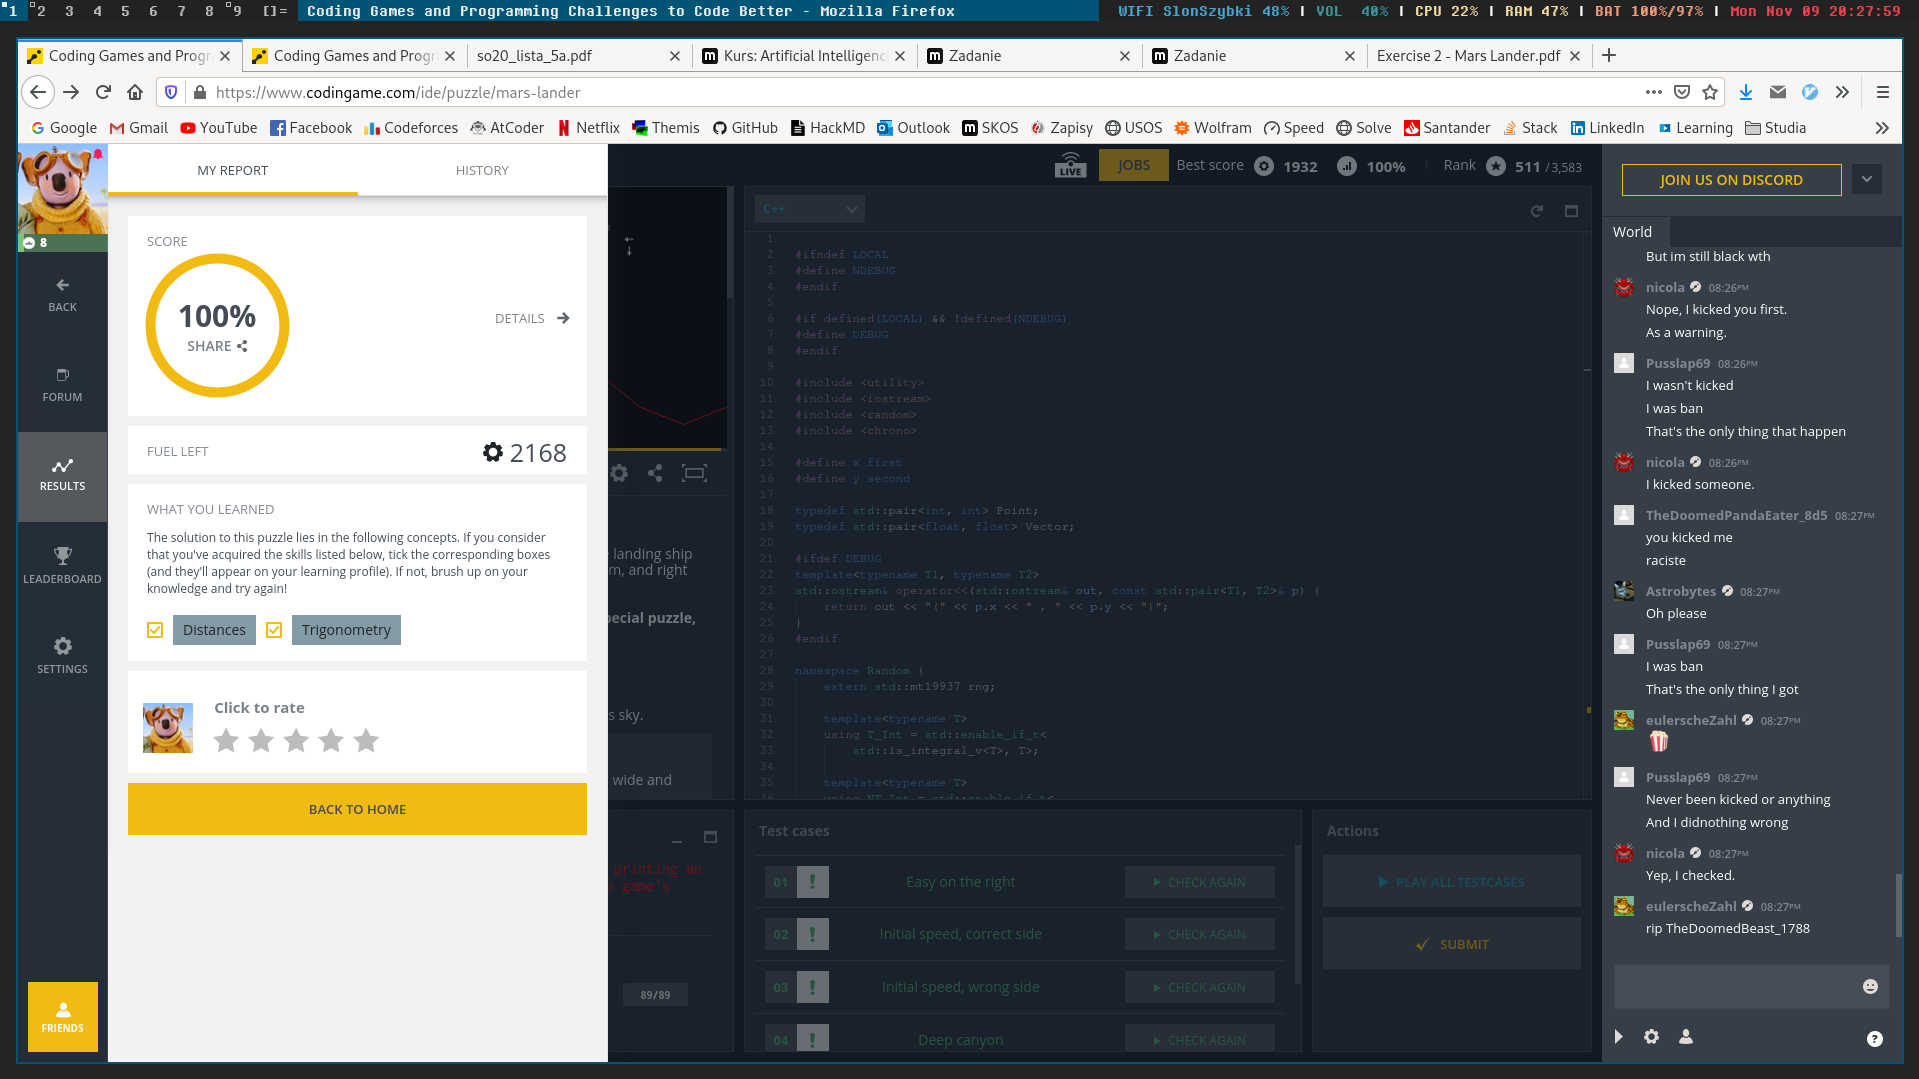
\includegraphics[scale=0.35]{screens/mars-lander-episode2} 	
	\caption{Proof of passing all the test cases and validators.}
 	\end{figure}
	
	When it comes to the evolutionary algorithm itself, I have tried a few different things. Firstly I have implemented RHEA algorithm with \textit{random gene mutation} and \textit{roulette wheel with elitism} selection. For crossover I have decided to try \textit{random weighted sum of two parents} as tried in the  Mars Lander blog.
	
	\begin{itemize}
		\item \textit{random gene mutation} - with small probability we choose a child and replace one of his genes with a random one
		\item \textit{roulette wheel with elitism} - we choose, e.g. \textit{20\%} of the best individuals of the current population and \textit{80\%} of the individuals using roulette wheel as parents for the next population
	\end{itemize}
	
	To make sure that I have implemented RHEA correctly, at first I have implemented simple evaluation function - as \textit{walk distance} between our current position and the middle point of the landing zone, where \textit{walk distance} is calculated as the distance on the land (if we are still flying I take the first point on the Mars ground looking directly below us). This way I could easily test if my algorithm works correctly - lander should try to get to the middle of the landing zone at all cost, considering neither fuel nor velocity.
	
	\subsection{Mutation}
	
	After a lot of debugging and testing a few parameters (I have also implemented visualization of my algorithm in SFML which helped me greatly) I saw, that my mutation was way to weak to properly explore the search space, so I had to tune the mutation parameter really high. But high mutation rate defeats the concept of mutation so I have decided to replace it with a different one - instead of deciding if I should mutate the given individual and then mutating one of his genes, for every individual and for all of his genes I mutated them independently with a small mutation probability. This way the mutations were much more meaningful - they really changed the behavior of the individual, as opposed to one gene mutation which really did not change the path of lander too much. I have also tried mutation which with small probability replaces the whole individual with a random one or "negates" him (changing angles to opposite) - although they were better than the first mutation, they lost with the second approach (independently mutating every gene).
	
	\subsection{Selection}
	One thing that I also saw to improve the convergence of the algorithm was to use \textit{elitism} in a slightly different way (it may be the original usage of elitism, which I think I did not understand at first) - instead of selecting let's say $20\%$ of the best individuals as parents and the rest of the parents with roulette wheel, I have just copied $20\%$ of the best individuals to the next population and then produced $80\%$ of the next population with roulette wheel and crossover. This approach (elitism as copying) was one of the main mechanism that drove the algorithm to the solution. It is also important to point out that \textit{elitismFactor}, which indicated how many individuals were copied , if too high will lead to the quick death of the population (it will consist only of the same individuals). If on the other hand \textit{elitismFactor} is too low, our population will not find the solution, as the search will be too random.
	
	\subsection{Crossover}
	After some tests I have also found out that \textit{single-point} crossover did better that \textit{random weight} crossover. I have also given a try to the \textit{uniform} crossover, which turned out the be the best of all the crossovers for me so I stuck with that. I suppose that when it comes to path-finding, shuffling the segments of the chromosomes from the parents could be really strong as we could imagine that the best path is some kind of merge of consecutive parts from two good parents. One could say that this crossover does not produce new values (it is just distributing the genes between two children), but I have represented the genes as the delta value of angle ($[-15,15]$) and delta value of thrust ($[-1,1]$), so effectively new values will be produced after such crossover. Moreover we cannot forget about the mutation which completes the circle.
	
	\paragraph{Link to the example evolutionary run of algorithm: }
	\href{https://gph.is/g/Z86B130}{EXAMPLE}
	
	\section{Fitness implementation}
	Fitness function was the most important part of the algorithm. Proper definition was the thing that made the Mars lander to properly land. I have specified five states that we would want to evaluate individual in (lander after actions in chromosome are done):\\
	
	\textit{Note:} I have decided to minimize the objective function and then transform it properly after the population evaluation so that the higher fitness, the better the individual.
		
	\begin{itemize}
		\item \texttt{Landed} - our destination, we take into the account remaining fuel - more fuel we have the better.
		\item \texttt{CrashedInside} - landing was not successful, so velocity (vertical and horizontal) above limit and non verical angle should be considered as a disadvantage. I also take into the account the distance from the middle of the landing zone, as sometimes position on CodingGame and in my program did not match and I thought I was in the landing zone when in reality I was outside it.
		\item \texttt{CrashedOutside} - the closer to the landing zone the better. Also really high speeds should be considered as a disadvantage.
		\item \texttt{Flying} - the same factors as for \texttt{CrashedOutside}, but treated slightly better than \texttt{CrashedOutside}.
		\item \texttt{FuelLack} - the worst state. That individual should really be discarded as it is probably not useful for others to inherit from the lander that ran out of fuel (at least in our examples).
	\end{itemize}
	
	The most important thing to note is that in all evaluations, the weights of all the elements taken into account are crucial. For example high speeds in \texttt{CrashedInside} should be of higher importance than high speeds in \texttt{Flying}. Also we should point out that, \texttt{Landed} $>$ \texttt{CrashedInside} $>$ \texttt{Flying} $>$ \texttt{CrashedOutside} $>$ \texttt{FuelLack} (inequalities hold to some degree, they are not that strict) and I have learned that it is important to make proper incentive for the population to strongly favor individuals that, e.g. \texttt{CrashedInside} from the ones that \texttt{CrashedOutside}. 
	
	From my experience making evaluation function not smooth when individual passes that states, helped to converge and find the solution (so for example crashing on the boundary of landing zone but outside it was noticeably worse from the evaluation function's perspective, than crashing inside the landing zone). That attitude could also be applied to high velocities. The individual with $41m/s$ vertical speed crashes inside the landing zone, but the individual with vertical speed that equals $40m/s$ can safely land, so I have tried to strongly differentiate between those similar velocities (one is just $1m/s$ higher than the other!). To do that I have added step values, when traversing between states or changing velocity from high to small (or vice-versa) as a reward/punishment.
	
	With velocities I have also used non linear functions (as $x^2$ or $x^3$) to reward the changes in velocity, especially if it is on the boundary of being high/low.
	
	\section{Final challenge}
	I have already described what I have tried, what worked and what did not or what I took into the account when evaluating the individual. When it comes to the final parameters I chose:
	\begin{enumerate}
		\item[] \texttt{Selection}: \textit{elitism + roulette wheel}
		\item[] \texttt{Crossover}: \textit{uniform crossover}
		\item[] \texttt{Mutation}: \textit{independent genes mutation}
		\item[] \texttt{Mutation probability}: $0.03$
		\item[] \texttt{Elitism factor}: $20\%$
		\item[] \texttt{Time for move}: $100ms$
	\end{enumerate}
	
	 \begin{figure}[h]
 	\centering
	
\includegraphics[scale=0.3]{screens/mars-lander-episode3} 	
	\caption{Proof of passing all the test cases and validators for episode 3.}
 	\end{figure}
 	
 	\section{Bonus score}
	\begin{figure}[H]
 	\centering
	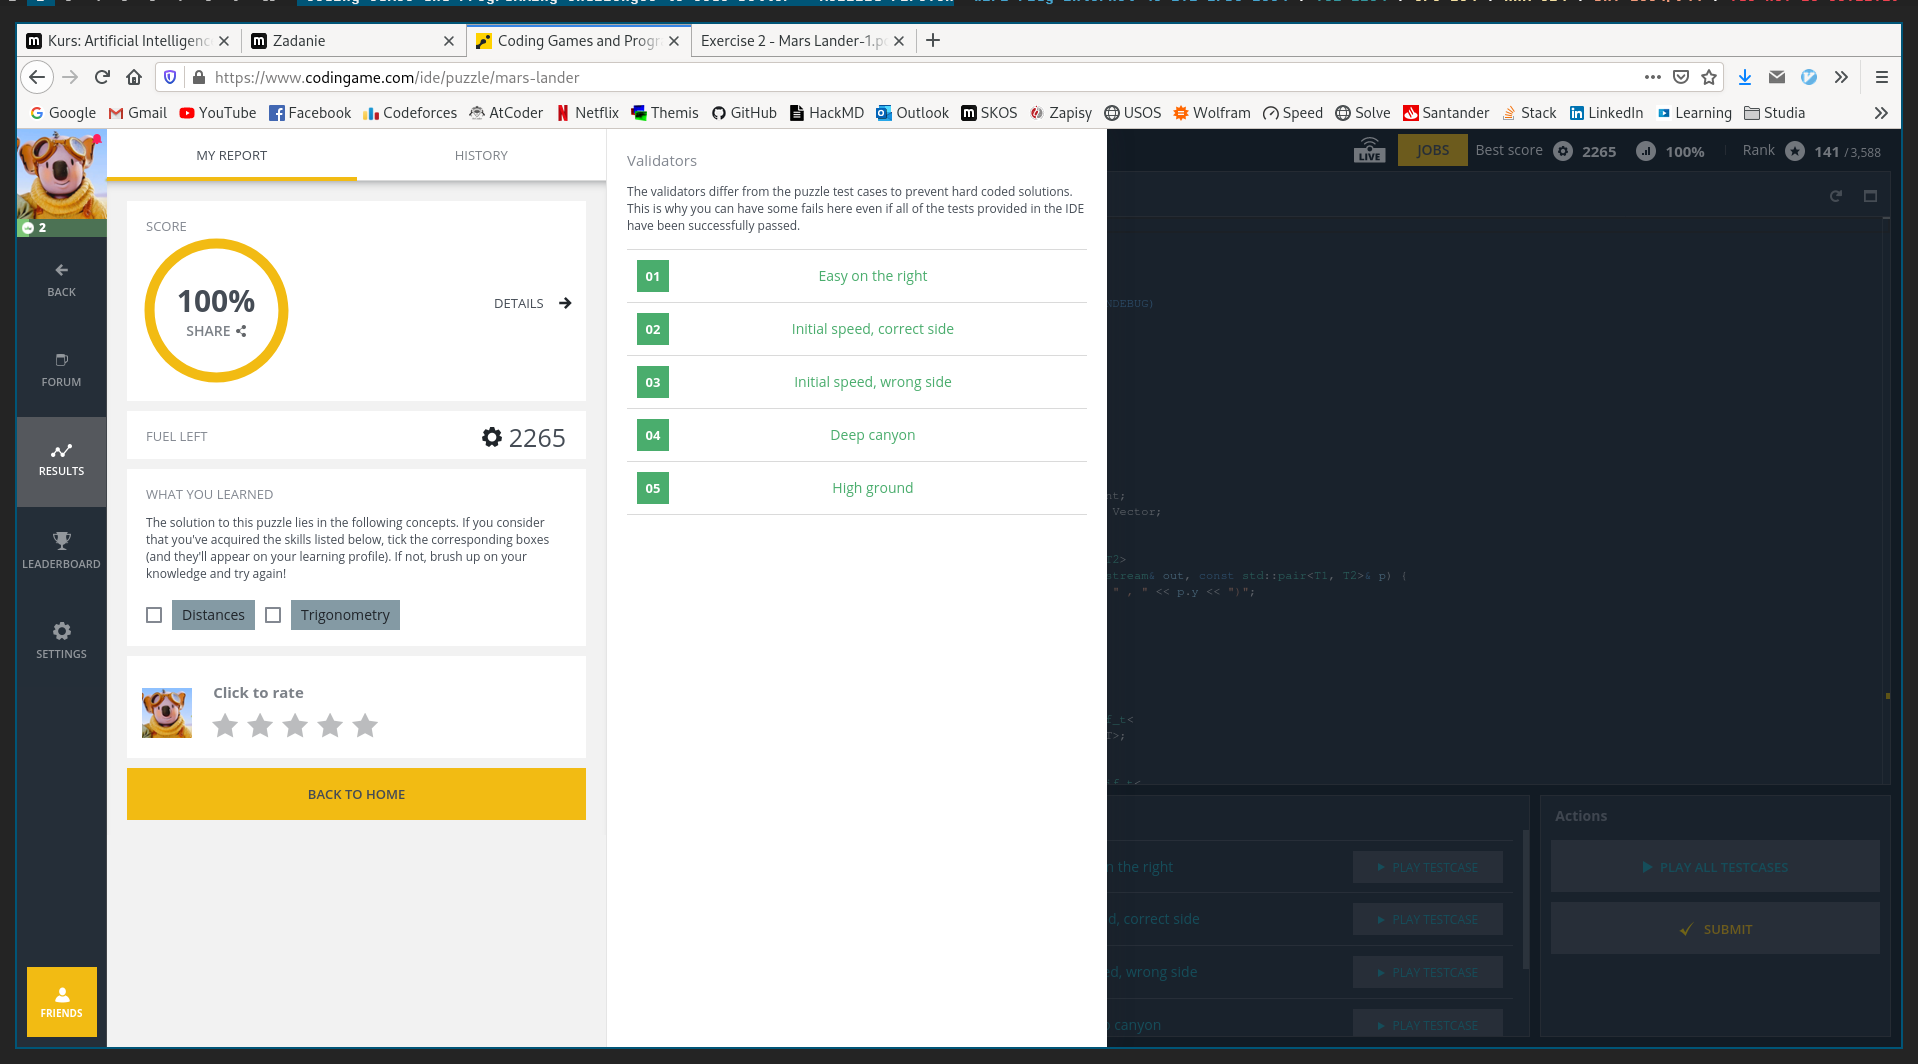
\includegraphics[scale=0.3]{screens/mars-lander-episode2-1} 	
	\caption{The best score I have managed to achive for episode 2.}
 	\end{figure}
 	
 	\begin{itemize}
 		\item[] \texttt{Best score}: $2265$
 		\item[] \texttt{CodingGame nickname}: nan0S\_\_
 	\end{itemize}
 	\textit{Note:} Although my main account nickname is nan0S\_ (yes, nan0S was taken), I had to create another one because on the original account I have reached 24h submission limit which I was not aware of.
 	
\end{document}
